\section{Allgemeines}
\setauthor{Lukas Starka}

\subsection{Rasa Produkte}
\setauthor{Lukas Starka}

Der Rasa Stack wird in Rasa NLU und Rasa Core aufgeteilt.
Diese sind so aufgebaut, dass sie unabhängig voneinander eingesetzt werden können.
So besteht die Möglichkeit, nur einen Teil der Architektur auf Rasa aufzubauen und zusätzlich weitere Services mit einzubinden.

\subsection{Rasa Core}
\setauthor{Lukas Starka}

Rasa Core ist verantwortlich für den Conversation Flow, Context-Handling, Bot-Responses und das Session Management.
Dabei kann auf der Rasa NLU oder anderen Services aufgebaut werden, die die Intent Recognition und Entity Extraction übernehmen und die Ergebnisse dem Rasa Core zur Verfügung stellen.\cite{rasaCore}

Rasa Core bezieht sich dabei auf die Hauptkomponente, die die Nachrichten erhält und darauf antwortet.\cite{rasaCore}

Der Rasa Core hält für jede Session, also für jeden User, einen Tracker.
Dieser enthält den momentanen Zustand der Konversationen, der jeweiligen User.
Bekommt der Bot nun eine Nachricht, wird zuerst der Interpreter durchlaufen, welcher den Originaltext als Eingabe bekommt, und die Eingabe, den Intent und die extrahierten Entities zurückgibt.
Zusammen mit dem aktuellen Zustand des Trackers entscheidet die Policy Komponente nun, welche Action, also Antwort des Bots, als nächstes ausgeführt werden soll.
Diese Entscheidung wird nicht durch einfache Regeln getroffen, sondern genauso wie Intents oder Entities, auf der Grundlage von einem, mit Machine Learning, trainierten Model.\cite{rasaCore, rasaCoreBook}

\begin{figure}[hbt!]
  \centering
  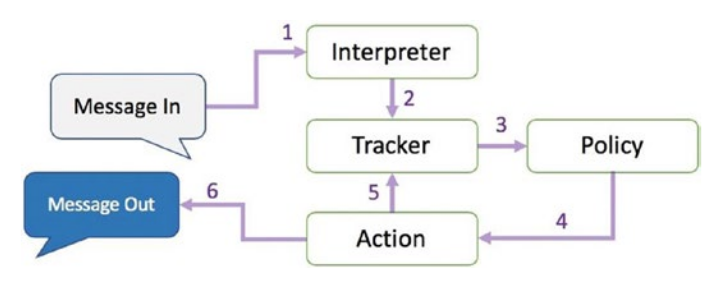
\includegraphics[scale=0.5]{pics/rasa-core}
  \caption{Rasa Core Aufbau~\cite{rasaCoreBook}}
  \label{fig:rasa_core}
\end{figure}

\subsection{Policies}
\setauthor{Lukas Starka}

Policies sind ein Teil von \textbf{Rasa Core} und der Assistent benützt Policies um zu entscheiden, welche Action als nächstes ausgeführt werden soll.
Es gibt machine-learning und rule-based policies.\cite{policies}

Hierbei kann man die Policies beispielsweise ändern.
Dies macht man in der \textbf{config.yml} Datei.

Bei den Policies gibt es unterschiedliche Priorities, die dann zum Einsatz kommen, wenn mehrere Policies dieselbe Confidence vorhergesagt haben.\cite{policyPriority}

\subsubsection{TED Policy}
\setauthor{Lukas Starka}

Die TED Policy steht für Transformer Embedding Dialogue Policy und wird meistens standardmäßig verwendet.\cite{tedPolicy}

Bei jedem Dialog bekommt die TED Policy drei Informationen als Input.
Die Nachricht des Users, die vorherige Action die vorhergesagt wurde und Slots und aktive Forms.
Dann werden diese in den Dialogue Transformer Encoder gepackt und anschließend werden sogenannte Dense Layer verwendet.
Danach wird die Ähnlichkeit zwischen den System Actions und dem Dialogue Embedding berechnet und zum Schluss werden noch CRF Algorithmen verwendet, um Entities zu erkennen.\cite{tedPolicy}



\subsection{Rasa NLU}
\setauthor{Lukas Starka}

Rasa NLU hat grundsätzlich zwei Hauptaufgaben.

Zum einen wäre da die Intent Recognition und die Entity Recognition.\cite{rasanlu, pretrainedVsSupervised}

Die Intent Recognition, ist die Erkennung der Nutzer-Absichten.
Dazu muss die NLU mit ausreichend Utterances, also Responses trainiert werden.
Dabei gibt die NLU alle zugehörigen Intents geordnet nach dem Confidence Score zurück.
Rasa verfügt demnach über ein Multi Intent Matching.\cite{rasanlu, pretrainedVsSupervised}

Außerdem gibt es noch die Entity Recognition, die dafür zuständig ist Entities, also wichtige Informationen, aus natürlicher Sprache zu extrahieren.\cite{rasanlu}

Der Aufbau der NLU ist vollständig konfigurierbar mithilfe der sogenannten Pipeline.\cite{howToChooseAPipeline}


\section{Pipeline}
\setauthor{Lukas Starka}
\label{sec:pipeline}

Rasa Open Source bietet bei der Initialisierung des Projekts eine Standard-NLU-Konfiguration.\cite{tuningYourModel}

In Rasa Open Source werden eingehende Nachrichten von einer Reihe von Komponenten verarbeitet.
Diese Komponenten werden nacheinander in einer sogenannten Processing Pipeline ausgeführt, die im config.yml File definiert ist.
Wenn man eine NLU-Pipeline auswählt, kann man allerdings sein Model anpassen und an das Dataset verfeinern.\cite{howToChooseAPipeline}

In der Abbildung 3 werden die Komponenten und ihre Lifecycle abgebildet.

\begin{figure}[hbt!]
  \centering
  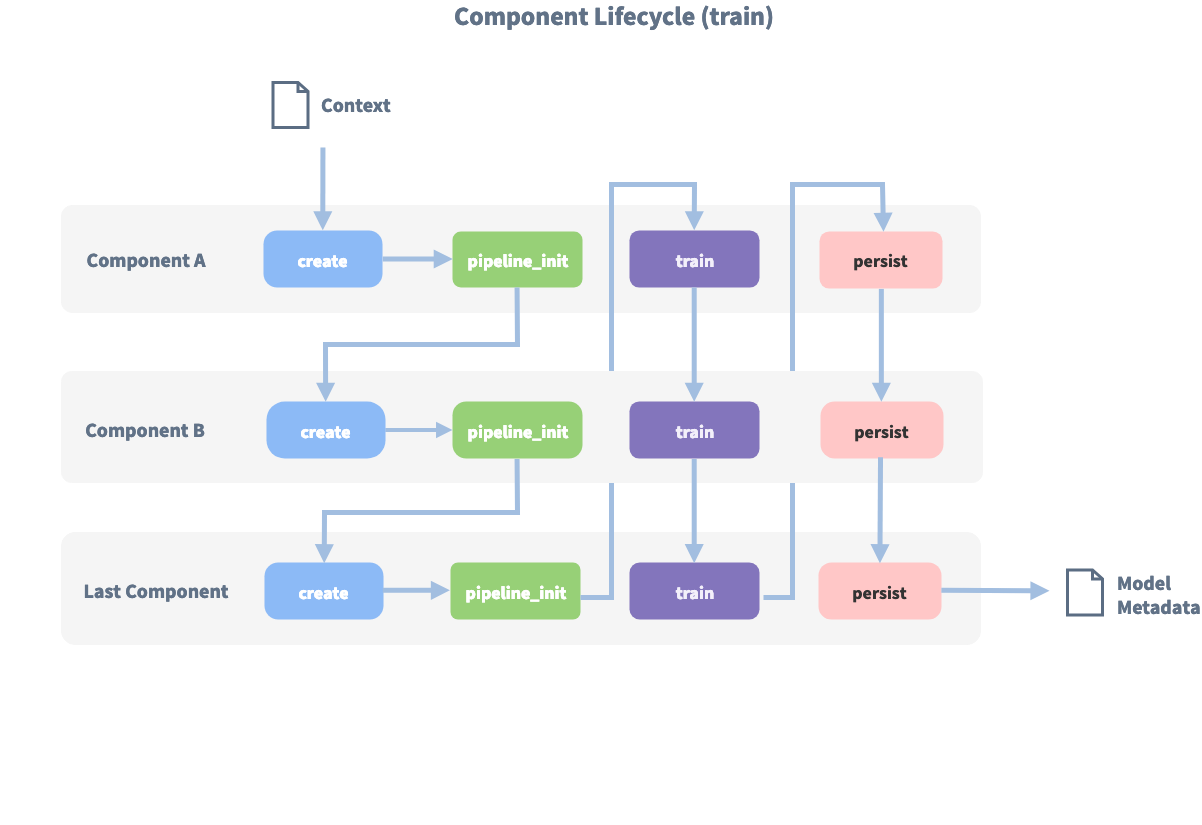
\includegraphics[scale=0.25]{pics/component-lifecycle}
  \caption{Component Lifecycle~\cite{componentLifecycle}}
  \label{fig:component_lifecycle}
\end{figure}

Bevor die erste Komponente mit der Create-Funktion erstellt wird, wird ein sogenannter Kontext erstellt (der nichts anderes als ein Python-dict ist).
Dieser Kontext wird verwendet, um Informationen zwischen den Komponenten zu übergeben.
Beispielsweise kann eine Komponente Merkmalsvektoren für die Trainingsdaten berechnen, diese im Kontext speichern und eine andere Komponente kann diese Merkmalsvektoren aus dem Kontext abrufen und eine Intent Klassifikation durchführen.\cite{componentLifecycle, componentLifecycleDoc}

Zunächst wird der Kontext mit allen Konfigurationswerten gefüllt, die Pfeile im Bild zeigen die Aufrufreihenfolge und visualisieren den Pfad des übergebenen Kontexts.
Nachdem alle Komponenten trainiert und beibehalten wurden, wird das finale context dictionary verwendet, um die Metadaten des Models beizubehalten.\cite{componentLifecycle, componentLifecycleDoc}

Dies ist in der Grafik 4 zu erkennen.

\begin{figure}[hbt!]
  \centering
  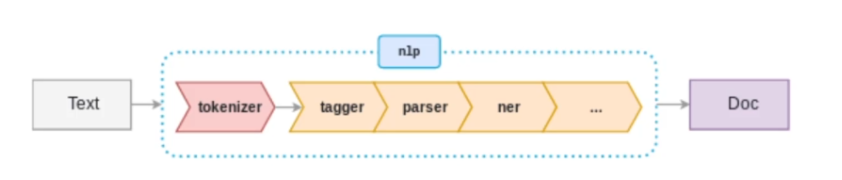
\includegraphics[scale=0.5]{pics/pipeline}
  \caption{Component Lifecycle~\cite{pipelineImage}}
  \label{fig:pipeline_image}
\end{figure}

\subsection{Arten von NLU Pipelines}
\setauthor{Lukas Starka}

Es gibt verschiedene bereits konfigurierte Pipelines.\cite{howToChooseAPipeline}

Grundsätzlich ist zwischen Pipelines zu unterscheiden, indem man sich informiert, ob sie pre-trained word vectors verwenden oder nicht.

\subsubsection{Beispiele für Pipelines mit pre-trained word vectors}

Der Vorteil von Pipelines, die pre-trained word vectors verwendet ist, dass diese bereits aus der jeweiligen Sprache word vectors besitzen.
Somit weiß das Model beispielsweise, dass Äpfel und Birnen ähnlich sind ohne, dass dies in den Intents irgendwo spezifiziert werden muss.\cite{differenceStackOverflow, rasaMasterclassPreConfiguredPipelines}

Die Vorteile hierbei sind also, dass das Model weniger Trainingsdaten benötigt, um eine gute Performance zu besitzen.
Außerdem geht der ganze Trainingsprozess in der Regel schneller und die sogenannten Iteration Times sind kürzer als bei Modellen ohne pre-trained word vectors.\cite{differenceStackOverflow, pretrainedVsSupervised, rasaMasterclassPreConfiguredPipelines}

\begin{lstlisting}[label={lst:spacy-sklearn-pipeline},caption={SpaCy Sklearn Pipeline}]{SpaCy Sklearn Pipeline}
language: "de"

pipeline: "spacy_sklearn"
\end{lstlisting}

Die SpaCy Pipeline verwendet pre-trained word vectors von GloVe oder fastText.\cite{spacySklearnPipeline, spacyNLP, rasaMasterclassPreConfiguredPipelines}

Es gibt außerdem auch noch Pipelines von MITIE.
Diese verwendet MITIE als Source für die word vectors.
Ein Vorteil von MITIE ist, dass man hier auch seine eigenen word vectors trainieren kann, indem man einen Corpus von Wikipedia oder ähnlichen Seiten verwendet.
Allerdings wird MITIE meistens nicht empfohlen und es könnte auch sein, dass MITIE demnächstet deprecated sein wird.\cite{mitieNLP, mitieDeprecated}

\begin{lstlisting}[label={lst:mitie-sklearn-pipeline},caption={MITIE Sklearn Pipeline}]{MITIE Sklearn Pipeline}
language: "de"

pipeline: "mitie_sklearn"
\end{lstlisting}

\subsubsection{Beispiele für Pipelines ohne pre-trained word vectors}

Der Vorteil von Pipelines ohne pre-trained word vectors ist, dass diese speziell auf den Fachbereich angepasst sind, für den man den Chatbot entwickelt.\cite{pretrainedVsSupervised, tensorFlowEmbedding}

Als Beispiel kann man die Wörter "balance" und "symmetry" aus dem Englischen sehen.
Diese Wörter sind eng miteinander verwandt.
Allerdings kann im Kontext von Banken das Wort "balance" auch mit "cash" verwandt sein.
Bei einem pre-trained Model würden diese Wortvektoren nicht nah aneinander liegen, aber wenn man einen Chatbot hat der nur Intents besitzt, die mit Banken und Rechnungswesen zu tun haben, werden diese zwei Wörter "balance" und "cash" ohne pre-trained word vectors als ähnlich erkannt werden.\cite{tensorFlowEmbedding}

Außerdem benutzen diese Pipelines kein sprach-spezifisches Model und somit kann man sie in allen Sprachen verwenden, die tokenisiert werden kann.\cite{tensorFlowEmbedding}


\begin{lstlisting}[label={lst:tensorflow-embedding-pipeline},caption={Tensorflow Embedding Pipeline}]{Tensorflow Embedding Pipeline}
language: "de"

pipeline: "tensorflow_embedding"
\end{lstlisting}

Der Bag-of-word-vectors Ansatz ist zwar sehr gut aber leider auch nicht perfekt.
Ein Problem davon ist, dass er oftmals keine fachspezifischen Begriffe kennt und außerdem können Typos nicht als Wortvektoren gelernt werden.
Außerdem ist das Problem bei pre-trained word vectors, dass zehntausende Vektoren gespeichert werden, die vermutlich nie verwendet werden.\cite{tensorFlowEmbedding, choosingPipeline}

Mit dem Tensorflow-Embedding macht man im Grunde genommen genau das Gegenteil.
Diese Pipeline verwendet keine pre-trained vectors und sollte mit jeder Sprache verwendet werden können.
Diese Pipeline lernt Embeddings für die Intents und für die Wörter und die Embeddings werden verwendet um die Ähnlichkeit zwischen dem Input und den Intents zu ermitteln.\cite{tensorFlowEmbedding, choosingPipeline}

Eine weitere Pipeline lautet wie folgt:

\begin{lstlisting}[label={lst:supervised-embedding},caption={Supervised Embedding Pipeline}]{Supervised Embedding Pipeline}
language: "de"

pipeline: "supervised_embedding"
\end{lstlisting}

\subsubsection{Supervised Embeddings vs. Pretrained Embeddings}

In der Grafik 5 sieht man ein Flussdiagramm, welches beschreibt, ob man Supervised Embeddings oder Pretrained Embeddings verwenden soll.

\begin{figure}[hbt!]
  \centering
  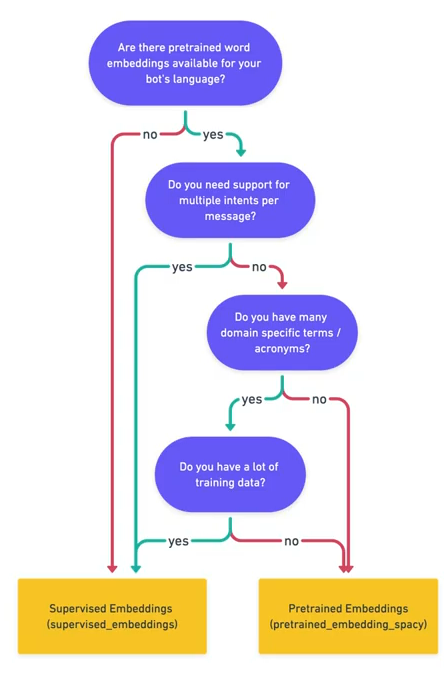
\includegraphics[scale=0.5]{pics/pre-trained-vs-supervised}
  \caption{Pretrained oder Supervised Embeddings~\cite{pretrainedVsSupervised, rasaMasterclassPreConfiguredPipelines}}
  \label{fig:pre_trained_vs_supervised}
\end{figure}

\subsection{Konfigurierte Pipelines}
\setauthor{Lukas Starka}

Es gibt also vordefinierte Pipelines von Rasa, die man nutzen kann.

Dabei kann man nun wieder entscheiden, ob man Pretrained Word Embeddings will oder nicht.
Sollte man sich dafür entscheiden, kann man auf eine Pipeline mit SpaCy zurückgreifen, welche den SpacyFeaturizer verwendet und somit Pretrained Word Embeddings nutzt.\cite{startingPipelines, allComponents}

\begin{lstlisting}[label={lst:spacy-pipeline},caption={Spacy Startpipeline}]{Spacy Startpipeline}
language: "de"  # Code für die Sprache

pipeline:
  - name: SpacyNLP
    model: "de_core_news_lg" # Spezifizierung, welches Modell von SpaCy genommen werden soll
  - name: SpacyTokenizer
  - name: SpacyFeaturizer
  - name: RegexFeaturizer
  - name: LexicalSyntacticFeaturizer
  - name: CountVectorsFeaturizer
  - name: CountVectorsFeaturizer
    analyzer: "char_wb"
    min_ngram: 1
    max_ngram: 4
  - name: DIETClassifier
    epochs: 100
  - name: EntitySynonymMapper
  - name: ResponseSelector
    epochs: 100

\end{lstlisting}

Wenn man sich dafür entscheidet keine vortrainierten Word Embeddings zu nutzen und somit sein Modell spezifischer auf den eigenen Anwendungsfall anpassen möchte, verwendet man die Standard Rasa Pipeline.
Diese verwendet den CountVectorsFeaturizer, bei dem nur die Trainingsdaten, die zur Verfügung gestellt werden, trainiert werden.\cite{startingPipelines, allComponents, nluExamples}

\begin{lstlisting}[label={lst:default-pipeline},caption={Default Pipeline}]{Default Pipeline}
language: "de"  # Code für die Sprache

pipeline:
  - name: WhitespaceTokenizer
  - name: RegexFeaturizer
  - name: LexicalSyntacticFeaturizer
  - name: CountVectorsFeaturizer
  - name: CountVectorsFeaturizer
    analyzer: "char_wb"
    min_ngram: 1
    max_ngram: 4
  - name: DIETClassifier
    epochs: 100
  - name: EntitySynonymMapper
  - name: ResponseSelector
    epochs: 100

\end{lstlisting}

Die von uns verwendete Pipeline beruht auf dieser Standard-Pipeline und die jeweiligen Komponenten werden in den folgenden Kapiteln genauer erläutert.

\begin{lstlisting}[label={lst:our-pipeline},caption={Unsere Pipeline}]{Unsere Pipeline}
language: de

pipeline:
   - name: WhitespaceTokenizer
   - name: RegexFeaturizer
   - name: LexicalSyntacticFeaturizer
   - name: CountVectorsFeaturizer
   - name: CountVectorsFeaturizer
     analyzer: char_wb
     min_ngram: 1
     max_ngram: 4
   - name: DIETClassifier
     epochs: 100
     constrain_similarities: true
   - name: EntitySynonymMapper
   - name: ResponseSelector
     epochs: 100
     retrieval_intent: faq
   - name: ResponseSelector
     epochs: 100
     retrieval_intent: chitchat
   - name: FallbackClassifier
     threshold: 0.3
     ambiguity_threshold: 0.1
\end{lstlisting}

\subsection{WhitespaceTokenizer}
\setauthor{Lukas Starka}

Ein WhitespaceTokenizer ist eine sehr einfache Art eines Tokenizers.
Hierbei wird, wie der Name bereits vermuten lässt, der Satz aufgeteilt in verschiedene Tokens.
Ein Token kann zum Beispiel also ein Wort sein und beim WhitespaceTokenizer wird der Satz pro Whitespace also Leerzeichen aufgeteilt.\cite{whitespaceTokenizer, rasaMasterclassWhitespaceTokenizer, pipelineComponentsYoutube}

\begin{figure}[hbt!]
  \centering
  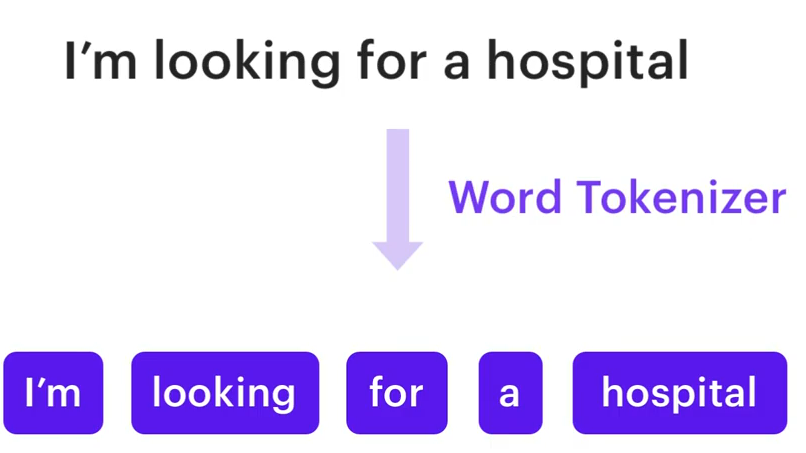
\includegraphics[scale=0.25]{pics/whitespacetokenizer}
  \caption{Tokens durch einen WhitespaceTokenizer~\cite{pipelineComponentsYoutube}}
  \label{fig:WhitespaceTokenizer}
\end{figure}

Es gibt auch komplexere Tokenizer und Tokenizer, die speziell an Sprachen angepasst sind und die besonderen Regeln, die in diesen Sprachen gelten, beachten.
Außerdem kann man natürlich auch selber einen Tokenizer schreiben.\cite{whitespaceTokenizer, rasaMasterclassWhitespaceTokenizer, pipelineComponentsYoutube}

Tokenizer sollten generell weit am Anfang einer Pipeline sein, wenn nicht sogar die erste Komponente.

\subsection{RegexFeaturizer}
\setauthor{Lukas Starka}

Einen RegexFeaturizer kann man verwenden, um die EntityExtraction zu erleichtern.
Bei diesem werden Regular Expressions und Lookup Tables verwendet und der RegexFeaturizer gibt an, ob ein Wort von den Regular Expressions oder Lookup Tables erkannt wurde.
Der EntityExtractor nimmt dann diese Tokens als Input und produziert Named Entity Recognition Ergebnisse.\cite{rasaMasterclassRegexFeaturizer, pipelineComponentsYoutube, regexFeaturizerCrf}

\subsubsection{Regular Expressions}

Regular Expressions können verwendet werden, um Muster eines Strings zu beschreiben und können hier bei dem Beispiel von Chatbots beispielsweise verwendet werden, um Zahlen zu beschreiben.\cite{rasaMasterclassRegexFeaturizer, pipelineComponentsYoutube, regexFeaturizerCrf}

\begin{figure}[hbt!]
  \centering
  
\includegraphics[scale=0.5]{pics/regular-expression-example}
  \caption{Regular Expression Beispiel~\cite{pipelineComponentsYoutube}}
  \label{fig:Regular Expression Beispiel}
\end{figure}

\subsubsection{Lookup Tables}

Lookup Tables können verwendet werden, wenn eine Entity vordefinierte Werte haben kann.
Zum Beispiel kann eine Entity mit dem Namen "country" 194 verschiedene Länder annehmen.\cite{rasaMasterclassRegexFeaturizer, pipelineComponentsYoutube, regexFeaturizerCrf}

\begin{figure}[hbt!]
  \centering
  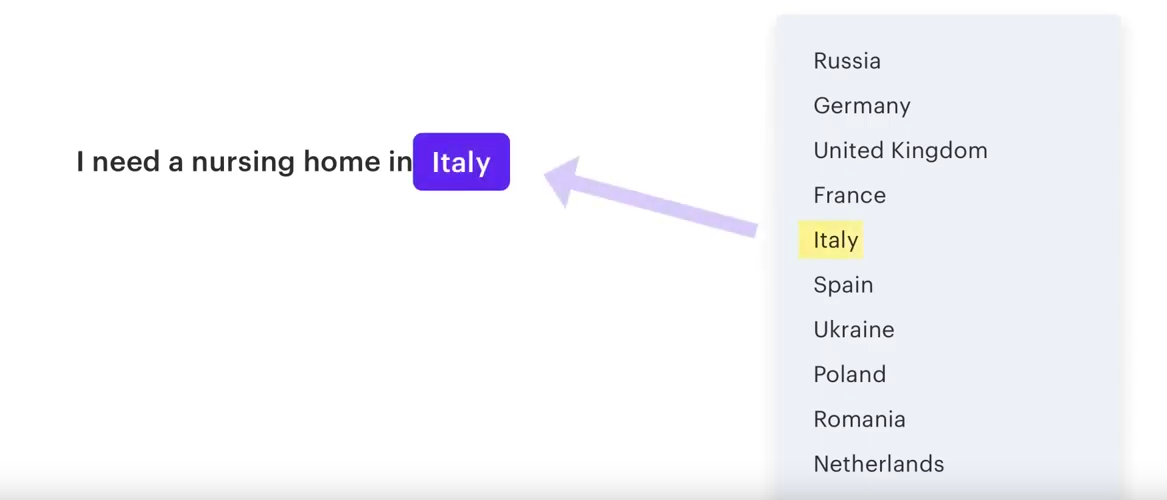
\includegraphics[scale=0.25]{pics/lookup-table-example}
  \caption{Lookup Table Beispiel~\cite{pipelineComponentsYoutube}}
  \label{fig:Lookup Table Beispiel}
\end{figure}

Der RegexFeaturizer muss vor dem EntityExtractor in der Pipeline platziert werden.\cite{rasaMasterclassRegexFeaturizer, pipelineComponentsYoutube, regexFeaturizerCrf}

\subsection{CRFEntityExtractor}
\setauthor{Lukas Starka}

Eine Möglichkeit um Entities aus der Nachricht des Benutzers zu extrahieren ist über den CRFEntityExtractor.\cite{crfEntityExtractor}

CRF steht hierbei für Conditional Random Field.
Dieses Modell lernt, welche Komponenten eines Satzes Entities sind und welche Entities diese sind.\cite{crfEntityExtractor, pipelineComponentsYoutube, regexFeaturizerCrf}
\ci
Dies macht der CRFEntityExtractor, indem er die Sequenzen der Tokens beobachtet.
Es wird also ein Token aus dem Satz herausgepickt, und anschließend wird geschaut, ob die Wörter danach und davor zum Kontext des Worts beitragen, um zu erkennen, ob es sich hierbei um eine Entity handelt.
Dabei schaut der Extractor auf Eigenschaften, wie beispielsweise, ob das Wort groß- oder kleingeschrieben ist, ob es einen Prefix hat, ob es eine Zahl ist oder ob es ein speziell definiertes Wort für die Entities ist.
Dies wird auch mit den Wörtern davor und danach gemacht.\cite{crfEntityExtractor, pipelineComponentsYoutube, regexFeaturizerCrf}

\begin{figure}[hbt!]
  \centering
  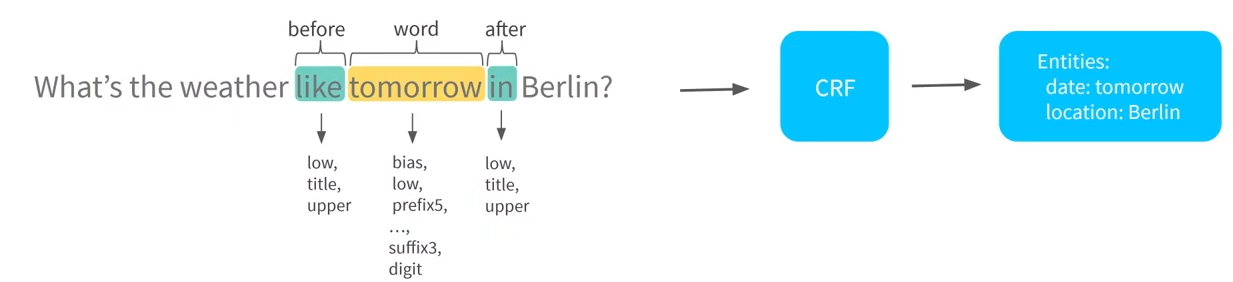
\includegraphics[scale=0.4]{pics/crf-entity-extractor}
  \caption{Funktionsweise vom CRFEntityExtractor~\cite{pipelineComponentsYoutube}}
  \label{fig:CRFEntityExtractor}
\end{figure}

Der CRFEntityExtractor produziert anschließend als Output, welche Wörter in einem Satz Entities sind und welche Entities diese sind, also was ihre Labels sind.
Außerdem wird noch produziert, wie sicher das Modell war, dass diese Entities korrekt sind, also die sogenannte Confidence wird ausgegeben und welches Modell verwendet wurde.\cite{crfEntityExtractor, pipelineComponentsYoutube, regexFeaturizerCrf}

\subsection{LexicalSyntacticFeaturizer}
\setauthor{Lukas Starka}

Ein Featurizer generell wird verwendet, um Features von den Tokens zu extrahieren.
Diese können dann von dem Intent-Klassifikations-Modell genutzt werden, um Muster zu erkennen und anschließend den korrekten Intent vorherzusagen.\cite{lexicalSyntacticFeaturizer, pipelineComponentsYoutube, pipelineConfigurationVideo}

\begin{figure}[hbt!]
  \centering
  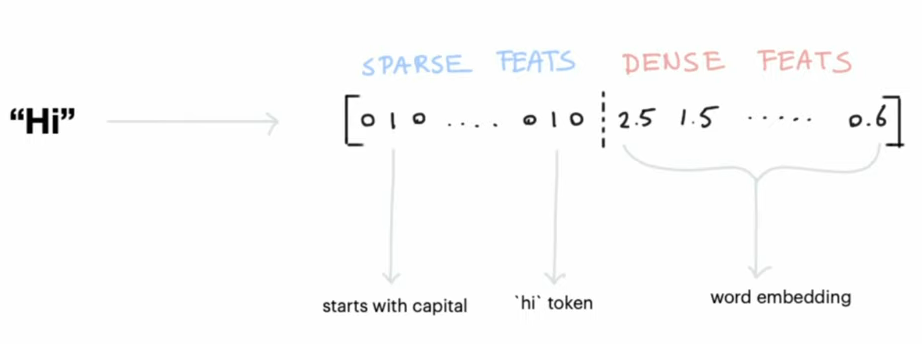
\includegraphics[scale=0.5]{pics/featurizer}
  \caption{Funktionsweise von einem Featurizer~\cite{pipelineConfigurationVideo}}
  \label{fig:Featurizer}
\end{figure}

Der LexicalSyntacticFeaturizer bekommt als Input einen Token und erstellt dann Features für die Entity Extraktion.
Dabei verwendet er ein sogenanntes Sliding Window, welches über jeden Token in der Nachricht des Benutzers verwendet wird.\cite{lexicalSyntacticFeaturizer, pipelineComponentsYoutube, pipelineConfigurationVideo}

\subsection{CountVectorsFeaturizer}
\setauthor{Lukas Starka}

Der CountVectorsFeaturizer erstellt Bag-of-Words.
Dabei wird gezählt, wie oft ein bestimmtes Wort aus den Trainingsdaten in der Nachricht des Benutzers vorkommt.
Dies wird dann als Input dem Intent-Classification-Model übergeben.\cite{countVectorsFeaturizer, pipelineConfigurationVideo, pipelineComponentsYoutube, rasaMasterclassCountVectorsFeaturizer}

\begin{figure}[hbt!]
  \centering
  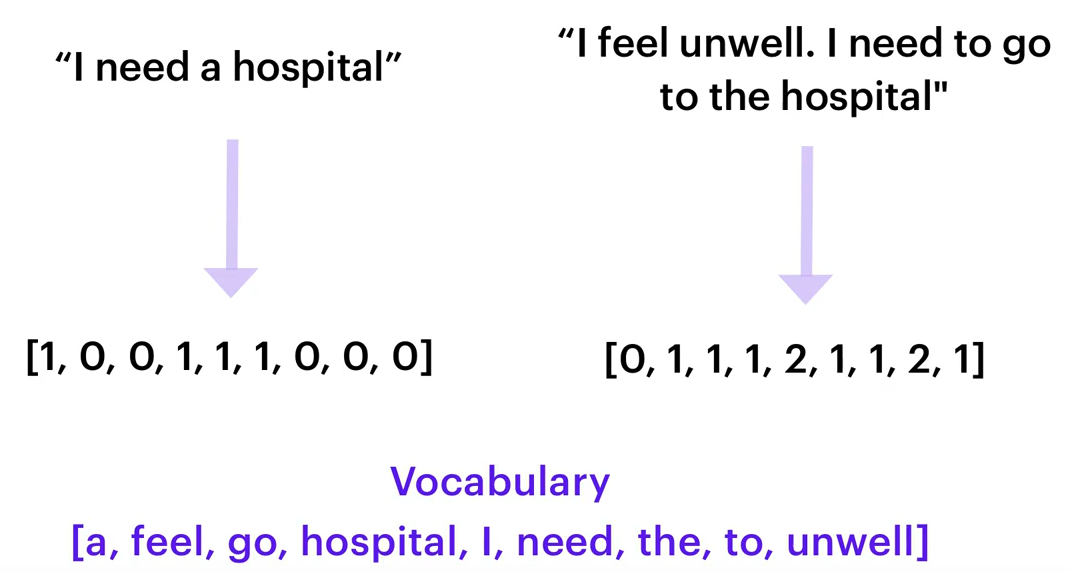
\includegraphics[scale=0.25]{pics/countvectorsfeaturizer}
  \caption{CountVectorsFeaturizer Beispiel~\cite{pipelineConfigurationVideo}}
  \label{fig:CountVectorsFeaturizer}
\end{figure}

Beim CountVectorsFeaturizer kann man außerdem angeben, dass statt Wörtern sogenannte n-grams verwendet werden sollen.
Dies macht das Modell in der Regel robuster gegen Typos allerdings erhöht sich damit auch die Zeit, die das Modell zum Trainieren benötigt.\cite{countVectorsFeaturizer, pipelineConfigurationVideo, pipelineComponentsYoutube, rasaMasterclassCountVectorsFeaturizer}

\begin{lstlisting}[label={lst:count-vectors-featurizer},caption={CountVectorsFeaturizer}]{CountVectorsFeaturizer}
pipeline:
    - name: CountVectorsFeaturizer
    analyzer: char_wb
    min_ngram: 1
    max_ngram: 4
\end{lstlisting}

\subsection{DIETClassifier}
\setauthor{Lukas Starka}

\subsection{EntitySynonymMapper}
\setauthor{Lukas Starka}

Der EntitySynonymMapper erwartet als Input einen Extractor von den Entity Extractors und liefert als Ausgabe modifizierte Werte für die Entities, die bereits vorher erkannt wurden.
Wenn beim EntitySynonymMapper also eine Entity überliefert wird und in den Trainingsdaten Synonyme für diese Entity vorhanden sind, wird der Wert der Entity auf den Wert, der in den Trainingsdaten angegeben ist, gesetzt.
Wenn also beispielsweise in einem Satz des Benutzers New York City oder NYC vorkommt, werden diese beide auf den selben Wert nyc gesetzt.\cite{entitySynonymMapper}

\begin{lstlisting}[label={lst:entity-synonym-mapper},caption={Entity Synonym Mapper}]{Entity Synonym Mapper}
[
    {
      "text": "I moved to New York City",
      "intent": "inform_relocation",
      "entities": [{
        "value": "nyc",
        "start": 11,
        "end": 24,
        "entity": "city",
      }]
    },
    {
      "text": "I got a new flat in NYC.",
      "intent": "inform_relocation",
      "entities": [{
        "value": "nyc",
        "start": 20,
        "end": 23,
        "entity": "city",
      }]
    }
]
\end{lstlisting}

\subsection{ResponseSelector}
\setauthor{Lukas Starka}

Ein Selector sagt die korrekte Response voraus aus einer Menge von möglichen Responses.
Beim ResponseSelector wird als Ausgabe ein Key-Value Paar ausgegeben.
Als Key wird hierbei der Retrieval Intent ausgegeben und das Value ist die vorhergesagte Response und die Confidence, mit der diese vorhergesagt wurde.\cite{responseSelector}

\begin{lstlisting}[label={lst:response-selector},caption={Response Classifier}]{Response Selector}
{
    "response_selector": {
      "faq": {
        "response": {
          "id": 1388783286124361986,
          "confidence": 0.7,
          "intent_response_key": "chitchat/ask_weather",
          "responses": [
            {
              "text": "It's sunny in Berlin today",
              "image": "https://i.imgur.com/nGF1K8f.jpg"
            },
            {
              "text": "I think it's about to rain."
            }
          ],
          "utter_action": "utter_chitchat/ask_weather"
         },
        "ranking": [
          {
            "id": 1388783286124361986,
            "confidence": 0.7,
            "intent_response_key": "chitchat/ask_weather"
          },
          {
            "id": 1388783286124361986,
            "confidence": 0.3,
            "intent_response_key": "chitchat/ask_name"
          }
        ]
      }
    }
}
\end{lstlisting}

Bei einem Retrieval Intent handelt es sich um einen speziellen Intent, der weiter aufgeteilt werden kann in sogenannte Sub-Intents.
Dies kann man zum Beispiel nutzen, wenn man einen Retrieval Intent für FAQ und für Chitchat hat, bei denen dann jede individuelle Frage einen Sub-Intent darstellt.\cite{retrievalIntent}
Verwendet wird dies, wenn der Bot zum Beispiel bei FAQ oder Chitchat sowieso immer mit der selben Antwort auf die Frage antworten soll, unabhängig von dem was vorher geschrieben wurde.\cite{chitchatAndFaqs}

Auch wir haben diesen Ansatz in unsere Pipeline gewählt.

\begin{lstlisting}[label={lst:response-selector-2},caption={Response Selector für Chitchat und FAQ}]{Response Selector}
- name: ResponseSelector
     epochs: 100
     retrieval_intent: faq
   - name: ResponseSelector
     epochs: 100
     retrieval_intent: chitchat
\end{lstlisting}

\subsection{FallbackClassifier}
\setauthor{Lukas Starka}

Der FallbackClassifier ist standardmäßig nicht in der Rasa Pipeline enthalten und wurde von uns hinzugefügt.\cite{startingPipelines}

Diesen verwendet man, um mit Nachrichten umzugehen, bei denen nur eine sehr niedrige Confidence vorhergesagt wurde.
In diesem Fall wird dann ein Intent mit dem Namen "nlu\_fallback" vorhergesagt, welchen man dann behandeln kann, indem man beispielsweise als Antwort immer definiert, dass der User seine Nachricht neu formulieren soll.
Die Confidence wird hierbei auf den Wert gesetzt welcher im Threshold angegeben wird.\cite{fallbackClassifier, nluFallback}
Man kann außerdem einen sogenannten "ambiguity\_threshold" angeben.
Bei diesem wird der "nlu\_fallback" Intent vorhergesagt, wenn die zwei als wahrscheinlichst empfundenen Intents sich um weniger, als den ambiguity\_threshold in der Confidence unterscheiden.\cite{fallbackClassifier}

\begin{lstlisting}[label={lst:fallback-classifier},caption={Fallback Classifier}]{Fallback Classifier}
pipeline:
- name: FallbackClassifier
  threshold: 0.7
  ambiguity_threshold
\end{lstlisting}

\section{Welche Rolle spielen neuronale Netze in Rasa}
\setauthor{Lukas Starka}

Rasa selbst definiert 5 Stufen von AI\@.\cite{ai5Levels}

\begin{figure}[hbt!]
  \centering
  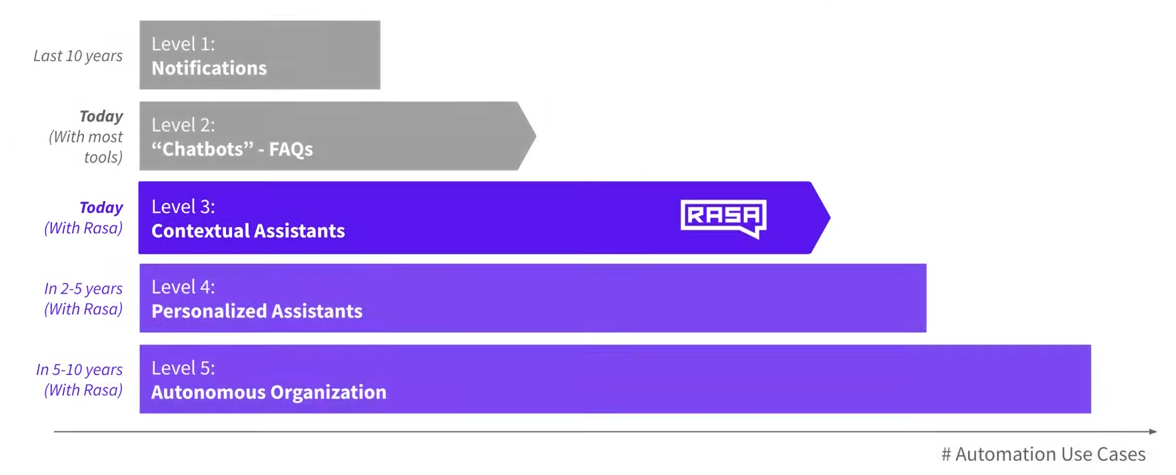
\includegraphics[scale=0.25]{pics/5_levels_of_ai}
  \caption{5 Stufen von AI~\cite{ai5LevelsVideo}}
  \label{fig:5_levels_of_ai}
\end{figure}

\textbf{Level 1: Notifications}

Auf Level 1 geht es darum simple Aufgaben zu erfüllen, wie man sie möglicherweise von seinem Smartphone kennt.
Darunter fällt zum Beispiel das Anlegen von Terminen und anderen Benachrichtigungen, die man dann zu der eingestellten Uhrzeit bekommt.\cite{rasaMasterclass5Levels,ai5Levels,ai5LevelsVideo}

\textbf{Level 2: "Chatbots" \& FAQs}

Auf Level 2 geht es darum, dass der Benutzer einfache Fragen stellen kann und anschließend der Chatbot auf diese antwortet.
Diese Stufe findet man sehr oft, allerdings sind diese sehr fehleranfällig, weil hier nur eine Menge an Regeln angelegt wird, an die sich der Chatbot hält.
Dies wird sehr oft in Form von FAQs genutzt und auch ein paar kleine Follow-up Fragen können hierbei schon definiert sein.\cite{rasaMasterclass5Levels,ai5Levels,ai5LevelsVideo}

\textbf{Level 3: Contextual AI Assistants}

Dieses Level wird derzeit von Rasa unterstützt.
Zusätzlich zu normalen FAQs wird hierbei auch der Kontext beachtet.
Es macht nämlich einen Unterschied, wann, wie und in welcher Situation ein Benutzer etwas gesagt hat.
Bei Contextual Assistants wird der Kontext, also was bereits zuvor gesagt wurde, auch beachtet.
Außerdem lenken sie Konversationen in die gewünschte Richtung und werden mit der Zeit immer besser, wenn man sie trainiert.\cite{rasaMasterclass5Levels,ai5Levels,ai5LevelsVideo}

\section{Komponenten}
\setauthor{Lukas Starka}

In der sogenannten Domain werden alle Intents, Entities, Slots, Responses, Forms und Actions angegeben, die der Bot kennt.
Diese ganzen Informationen befinden sich in der \textbf{domain.yml} Datei.\cite{domain}

\subsection{Intents}
\setauthor{Lukas Starka}

Intents sind die Absichten hinter der Nachricht des Benutzers.
Als Intents werden also alle möglichen Beispielsätze definiert, die ein Benutzer sagen könnte, um eine bestimmte Absicht auszudrücken.\cite{intents}

Intents werden in dem \textbf{nlu.yml} File wie folgt angegeben:

\begin{lstlisting}[label={lst:intent-example},caption={Intents Beispiel}]{Intents Beispiel}
## intent:<name des intents>
- <phrase 1>
- <phrase 2>
- <phrase 3>
\end{lstlisting}

\subsection{Responses}
\setauthor{Lukas Starka}

Responses sind die Antworten, die vom Bot gegeben werden, wenn ein bestimmter Intent erkannt wurde.\cite{responses}

Responses fügt man in seinem \textbf{domain.yml} File wie folgt ein:

\begin{lstlisting}[label={lst:responses-example},caption={Responses Beispiel}]{Responses Beispiel}
responses:
  utter_greet:
  - text: "Hey! How are you?"

  utter_<name der response>:
  - text: "<text>"
    image: "<img link>"
  ...
\end{lstlisting}


\subsection{Stories}
\setauthor{Lukas Starka}

Stories werden als Trainingsdaten verwendet, die zum Trainieren des Models des Bots verwendet werden.
Stories können dabei genutzt werden, um Models zu trainieren, bei denen auch unvorhersehbare Konversationspfade behandelt werden und unterscheiden sich in dieser Hinsicht von den Rules.
\cite{stories}

Bei einer Story wird also die Unterhaltung zwischen einem Benutzer und dem Bot dargestellt.
Dabei wird die Eingabe des Benutzers als Intent angegeben und die Antwort, mit der der Bot antworten soll, als Name der Action.\cite{stories}

Stories können wie folgt aussehen und sind im \textbf{stories.yml} File anzugeben:

\begin{lstlisting}[label={lst:stories-example},caption={Stories Beispiel}]{Stories Beispiel}
stories:
- story: name der story
  steps:
  - intent: <name des intents>
  - action: <name der action>
\end{lstlisting}

\subsubsection{Checkpoints und OR-Statements}

Man kann seine Stories außerdem mit Checkpoints und OR-Statements versehen.
Bei diesen sollte man aber grundsätzlich aufpassen und sie nur bedacht verwenden, weil in den meisten Fällen die gewünschten Resultate besser mit \textbf{Rules} oder einem \textbf{ResponseSelector} zu erzielen sind.
\cite{checkpointsor}

Checkpoints können genutzt werden, um seine Trainingsdaten zu vereinfachen, indem man einen Checkpoint in einer Story setzt und auf diesen in einer anderen Story wieder ansetzt.
Von diesen sollte man allerdings nicht zu viele machen, weil sonst die Stories sehr leicht schwer zu lesen und unübersichtlich sind und außerdem die Trainingszeit dadurch erhöht wird.
\cite{checkpoints}

Man definiert einen Checkpoint am Ende seiner Story, wenn man diesen Teil der Story auch wieder als Voraussetzung für eine weitere Story setzt.
In der nächsten Story beginnt man dann mit seinem Checkpoint, also dem Punkt auf den man anknüpfen möchte und die Teile der Konversation, die für diese Story ebenfalls vorausgesetzt werden sollen.

Im folgenden Beispiel werden Checkpoints von Stories verwendet, um an anderen Stories anzuknüpfen\cite{checkpoints}
:

\begin{lstlisting}[label={lst:checkpoints-example},caption={Checkpoints Beispiel}]{Checkpoint Beispiel}
stories:
- story: beginning of flow
  steps:
  - intent: greet
  - action: action_ask_user_question
  - checkpoint: check_asked_question

- story: handle user affirm
  steps:
  - checkpoint: check_asked_question
  - intent: affirm
  - action: action_handle_affirmation
  - checkpoint: check_flow_finished

- story: handle user deny
  steps:
  - checkpoint: check_asked_question
  - intent: deny
  - action: action_handle_denial
  - checkpoint: check_flow_finished

- story: finish flow
  steps:
  - checkpoint: check_flow_finished
  - intent: goodbye
  - action: utter_goodbye
\end{lstlisting}

OR-Statements können dafür verwendet werden, wenn man auf mehrere Intents innerhalb einer Story gleich reagieren möchte.\cite{orStatements}

Man schreibt also anstelle von einem Intent in der Story ein \textbf{or} und gibt darunter alle Intents an, von denen einer eintreffen muss, damit die Story zutrifft.

\begin{lstlisting}[label={lst:or-example},caption={OR Beispiel}]{OR Beispiel}
stories:
- story:
  steps:
  # ... vorherige schritte
  - action: utter_ask_confirm
  - or:
    - intent: affirm
    - intent: thankyou
  - action: action_handle_affirmation
\end{lstlisting}

\subsection{Rules}
\setauthor{Lukas Starka}

Rules werden angegeben, um kleine Teile von Unterhaltungen anzugeben, die immer wieder gleich behandelt werden sollen.
Diese sollten allerdings nicht allzu häufig verwendet werden, weil man nie alle Konversationen vorhersagen kann.
Um Rules verwenden zu können, muss man die \textbf{RulePolicy} in der Policy Konfiguration eintragen.\cite{rules}

Um eine Rule zu verwenden, schreibt man folgendes in sein \textbf{rules.yml} File:

\begin{lstlisting}[label={lst:rules-example},caption={Rules Beispiel}]{Rules Beispiel}
rules:

- rule: Say `hello` whenever the user sends a message with intent `greet`
  steps:
  - intent: greet
  - action: utter_greet
\end{lstlisting}

\subsection{Slots}
\setauthor{Lukas Starka}

Slots sind sozusagen das Gedächtnis des Bots.
Diese sind als key-value Paare dargestellt und können dazu verwendet werden, damit Information, die der Benutzer bereitstellt, gespeichert werden können, ähnlich zu Entities.
Diese Informationen können beispielsweise der Name des Benutzers sein oder Informationen, die für den generellen Kontext des Gesprächs wichtig sind.
\cite{slots}

\begin{lstlisting}[label={lst:slots-example},caption={Slots Beispiel}]{Slots Beispiel}
slots:
  slot_name: <slot name>
    type: <type>
\end{lstlisting}


\subsection{Entities}
\setauthor{Lukas Starka}

Entities sind strukturierte Stücke von Informationen, die sich innerhalb der Nachricht eines Benutzers befinden.
Solche Entities können beispielsweise ein Ort, ein Beruf oder ein Name sein.\cite{entities}

Um Entities zu erstellen schreibt man folgendes in sein \textbf{domain.yml} File:

\begin{lstlisting}[label={lst:entities-domain-example},caption={Entities in der Domain}]{Entities in der Domain}
entities:
  - <entity name>
  - <entity name>
\end{lstlisting}

Diese Entities müssen dann noch in den Intents angegeben werden, in denen sie vorkommen sollen.
Dies macht man, indem man folgende Syntax bei den Trainingssätzen im \textbf{nlu.yml} File verwendet und ergänzt:

\begin{lstlisting}[label={lst:entities-nlu-example},caption={Entities Beispiel}]{Entities Beispiel}
Hallo mein Name ist [Lukas](name).
Ich hätte gerne eine [kleine](size) [Pizza](meal)
\end{lstlisting}

\subsubsection{Entity Roles}

Entity Roles können sinnvoll in manchen Szenarien sein.
Zum Beispiel bei folgendem Satz:

\begin{lstlisting}[label={lst:entity-roles-example},caption={Entity Roles Beispiel}]{Entity Roles Beispiel}
Buche einen Flug von [Linz](city) nach [London](city).
\end{lstlisting}

In diesem Fall sind sowohl Linz als auch London zwar richtig gekennzeichnet als city Entity, allerdings reicht diese Information noch nicht aus, damit der Chatbot richtig reagieren kann.
Hierbei wäre es praktisch, wenn man noch angibt, welche dieser zwei Städte das Ziel und welche der Abflugsort ist.
Dies macht man mit Entity Roles.\cite{entityRolesGroups}

\subsubsection{Entity Groups}

Entity Groups können genutzt werden, wenn man Entities miteinander gruppieren möchte.\cite{entityRolesGroups}

Dies kann zum Beispiel hier sinnvoll sein:

\begin{lstlisting}[label={lst:entity-groups-example},caption={Entity Groups Beispiel}]{Entity Groups Beispiel}
Ich hätte gerne eine kleine [Pizza](meal) mit [Pilzen](topping) und eine [Salami](topping) [Pizza](meal).
\end{lstlisting}

Bei der Gruppe muss hier erkannt werden, welche zwei Entities zusammen gehören\cite{entityRolesGroups}:

\begin{lstlisting}[label={lst:entity-groups-example-2},caption={Entity Groups Beispiel 2}]{Entity Groups Beispiel 2}
Ich hätte gerne eine kleine [Pizza](meal) mit [Pilzen](topping) und eine [Salami](topping) [Pizza](meal).
Group 1: [Pizza](meal) [Pilzen](topping)
Group 2: [Salami](topping) [Pizza](meal)
\end{lstlisting}


\subsubsection{Nutzung von Entity Roles und Entity Groups}

\subsection{Actions}
\setauthor{Lukas Starka}

Es gibt 2 verschiedene Arten von Messages:

\begin{enumerate}
  \item \textbf{Static Messages}: Diese sind unabhängig vom User Input und benötigen keinen Action Server\cite{actionsVid}
  \item \textbf{Dynamic Messages}: Diese sind abhängig vom User Input und benötigen einen Action Server\cite{actionsVid}
\end{enumerate}

Der Rasa Action Server führt sogenannte Custom Actions für einen Rasa Open Source Conversation assistent aus.

Wenn der Assistant eine gewisse Custom Action vorhersagt, sendet der Rasa Server einen POST request an den Actionserver mit einer JSON Payload mit dem Namen der vorhergesagten Action, der Conversation ID, den Inhalten des Trackers und den Inhalten der Domain.\cite{actions}

\subsection{Forms}
\setauthor{Lukas Starka}

Um mehrere Informationen von einem Benutzer zu bekommen, eignen sich Forms.
Um Forms zu verwenden, muss die \textbf{RulePolicy} in der Policy Konfiguration eingetragen sein.\cite{forms}

Wenn man ein Formular hinzuzufügen will, muss man dies in der forms Section in dem \textbf{domain.yml} File angeben.

\begin{lstlisting}[label={lst:forms-example},caption={Forms Beispiel}]{Forms Beispiel}
forms:
  restaurant_form:
    required_slots:
        cuisine:
          - type: from_entity
            entity: cuisine
        num_people:
          - type: from_entity
            entity: number
\end{lstlisting}


\subsection{Synonyms}
\setauthor{Lukas Starka}

Mithilfe von Synonymen kann man extrahierten Entities einen anderen Wert geben, als sie eigentlich vorher hatten, wenn diese in der Bedeutung gleich sind.
Wenn man also mit verschiedenen Wörtern dasselbe meint, kann man sich Synonyms zur Hilfe nehmen.\cite{synonyms}

Ein Beispiel dafür wäre folgendes im \textbf{nlu.yml} File:

\begin{lstlisting}[label={lst:synonym-example},caption={Synonym Beispiel}]{Synonym Beispiel}
- synonym: Medientechnik
  examples: |
    - IT-Medientechnik
    - IT Medientechnik
    - Medientechnologie
\end{lstlisting}

\subsection{Custom Actions}
\setauthor{Lukas Starka}

\section{Initialisieren}
\setauthor{Lukas Starka}

\subsection{Rasa Init}
\setauthor{Lukas Starka}

Einen neuen Rasa Assistant kann man mithilfe des Init-Befehls in der Konsole anlegen.
Der Befehl dafür lautet wie folgt:

\begin{lstlisting}[language=bash,label={lst:init-example},caption={Befehl fürs Initialisieren}]{Rasa Init Befehl}
rasa init
\end{lstlisting}

Bei diesem Befehl wird man gefragt, ob man direkt ein voreingestelltes Model trainieren möchte.
Dieses Modell wird basierend auf den Demodaten, die von jedem neu erstellten Rasa Projekt zur Verfügung gestellt werden, trainiert.

\begin{figure}[hbt!]
  \centering
  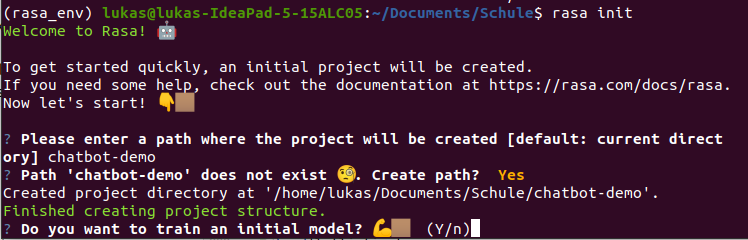
\includegraphics[scale=0.5]{pics/rasa_init}
  \caption{Rasa Init Konsolenausgabe}
  \label{fig:rasa_init}
\end{figure}

Nachdem dieser Befehl ausgeführt wurde, bekommt man folgende Files, die für einen Chatbot benötigt werden.

\begin{figure}[hbt!]
  \centering
  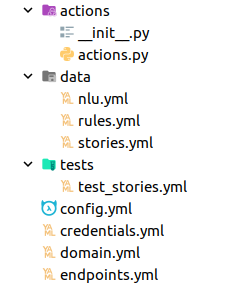
\includegraphics[scale=0.75]{pics/rasa_file_tree}
  \caption{File Tree nach dem Initialisieren}
  \label{fig:file_tree}
\end{figure}

\section{Trainieren}
\setauthor{Lukas Starka}

\subsection{Rasa Train}
\setauthor{Lukas Starka}

Um das Modell nun zu trainieren nützt man den \texttt{Rasa train} Befehl.

\section{Interagieren}
\setauthor{Lukas Starka}

\subsection{Rasa Shell}
\setauthor{Lukas Starka}

Wenn man sich nun mit seinem Bot unterhalten möchte, kann man eine Chat Session über die Konsole mit dem \texttt{rasa train} Befehl.
Normalerweise wird dabei das aktuellste Modell genommen.
Sollte man dies allerdings nicht wollen, kann man mit \texttt{--model} auch den Pfad zum richtigen Modell angeben.

\begin{lstlisting}[language=bash,label={lst:shell-command},caption={Rasa Shell Befehle}]{Rasa Shell}
rasa shell
rasa shell --model models/20220211-094939.tar.gz
rasa shell --debug
\end{lstlisting}

Für detailliertere Ausgaben kann man außerdem das \texttt{--debug} Flag verwenden.
Die Ausgabe dabei sieht wie in Abbildung~\ref{fig:rasa_shell} aus:

\begin{figure}[hbt!]
  \centering
  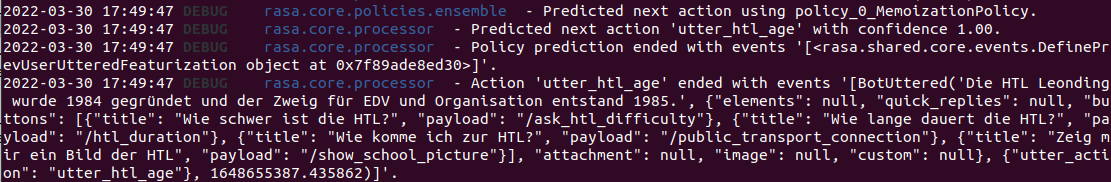
\includegraphics[scale=0.40]{pics/rasa_shell}
  \caption{Rasa Shell Ausgabe mit Debug Flag}
  \label{fig:rasa_shell}
\end{figure}

\subsection{Rasa Interactive}
\setauthor{Lukas Starka}

Um eine interaktive Session mit dem Bot zu starten, kann man den Befehl \texttt{rasa interactive} nutzen.
Dabei wird zunächst ein Modell trainiert und anschließend startet eine interaktive Shell Session.
Dabei kann man dann alle vorhergesagten Aktionen vom Assistant korrigieren.
Wenn man nur das Core Model testen möchte, kann man dies spezifizieren.

\begin{lstlisting}[language=bash,label={lst:interactive-command},caption={Interaktive Trainingssession starten}]{Rasa Interactive}
rasa interactive
rasa interactive --model models/20220211-094939.tar.gz
rasa interactive core
\end{lstlisting}

Bei dieser Trainingssession hat man die Möglichkeit jedes Mal anzugeben, ob der vorhergesagte Intent und die daraus resultierende Antwort die richtige sind.
Außerdem wird die gesamte Chat History visualisiert und ausgegeben, wie in Abbildung ~\ref{fig:rasa_interactive} zu sehen ist.

\begin{figure}[hbt!]
  \centering
  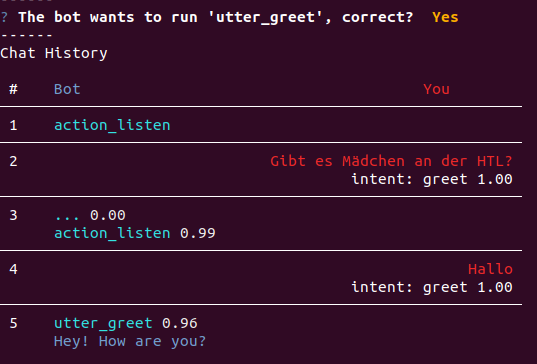
\includegraphics[scale=0.80]{pics/rasa_interactive}
  \caption{Ausgabe beim Interactive Befehl}
  \label{fig:rasa_interactive}
\end{figure}
